
We evaluate the performance of the proposed methodology for the task of human body pose correspondence estimation, as well as non-rigid alignment ``in-the-wild''. For further experimental results, please refer to the supplementary material.

%Results of quantitative and qualitative evaluations are reported.

\begin{figure}[t!]
    \centering
    \includegraphics[width=\columnwidth]{resources/Fig_Variance/final}
    % 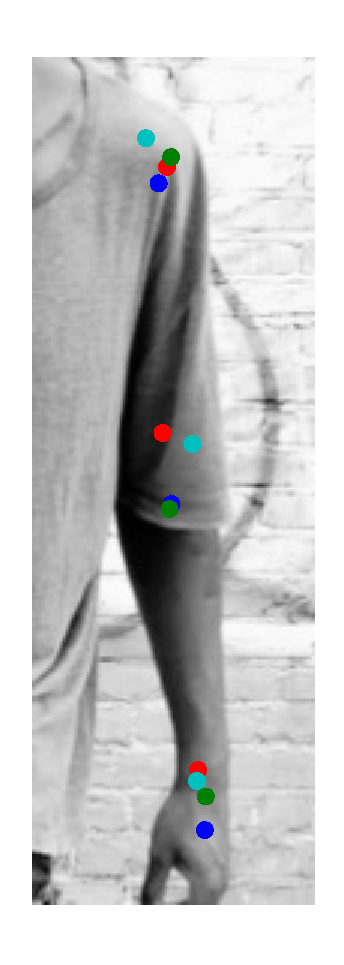
\includegraphics[height=\vfh]{resources/Fig_Variance/image_1}
    % 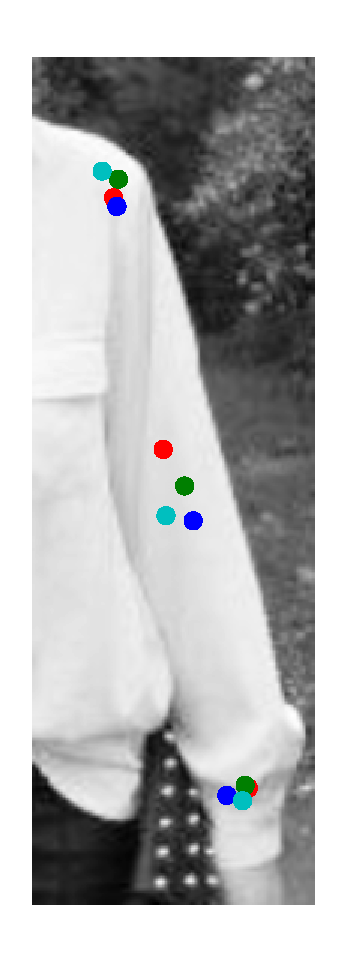
\includegraphics[height=\vfh]{resources/Fig_Variance/image_2}
    % 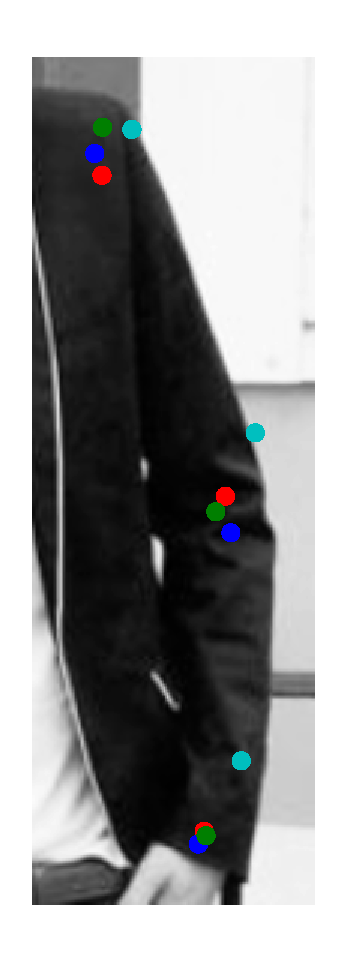
\includegraphics[height=\vfh]{resources/Fig_Variance/image_4}
    % 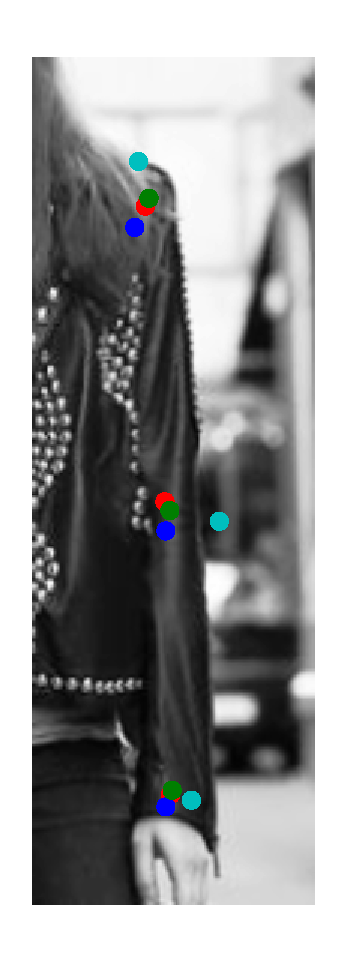
\includegraphics[height=\vfh]{resources/Fig_Variance/image_6}
    % 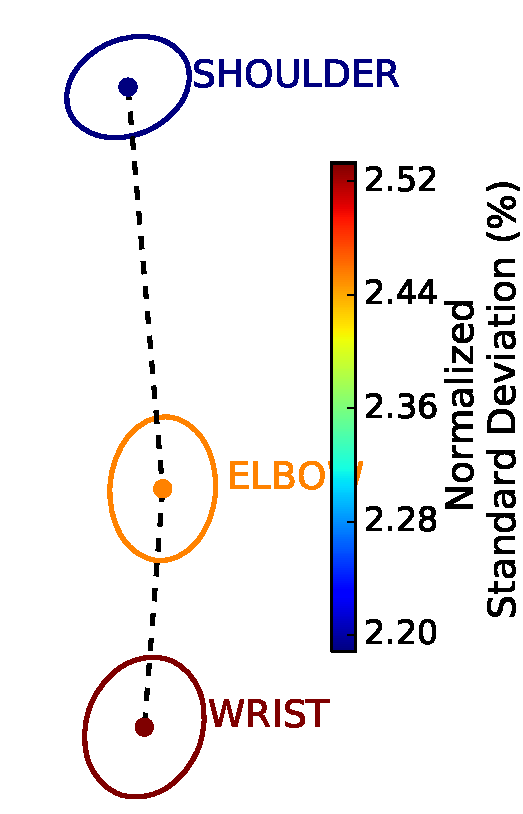
\includegraphics[height=\vfh]{resources/Fig_Variance/variances}
    \caption{Example of human pose annotation for left arm among 4 annotators. The large variance shows the difficulties of having consistent landmarks. Figure best viewed by zooming in.}
    \label{fig:variance}
\end{figure}





\subsection{Non-rigid Object Alignment In-the-wild}
\label{exp:daam_benchmark}
Herein, we compare the fitting accuracy of the dAAMs that are trained with our proposed framework with holistic sparse AAMs~\cite{Cootes2001,Matthews2004}. We consider two object classes that demonstrate rich texture: face and ear.


\paragraph{Databases \& Error Metrics} In the case of face, we build both models using the 811 training images of the Labelled Faces Parts in-the-Wild (LFPW) \cite{belhumeur2013localizing}. Sparse AAMs were built from the 68 points annotations provided by~\cite{sagonas_iccv_300w_2013}. Our dAAMs were built as described in Step~\ref{sec:step4}. In both cases we build the appearance models using pixel intensities. The results are reported on the 224 images of the LFPW testset.


In the case of the ear, given the lack of publicly available annotated databases, we collected 605 high resolution images from the internet, that were captured under unconstrained conditions. The images were manually annotated with respect to a 55 point sparse annotation mark-up, as well as the curve annotations proposed in this paper. Examples of these two type of ear annotations are shown in Figure \ref{fig:intro}. We randomly split the database into two disjoint sets of training (500) and testing (105) images. The training of the two models was done in the same way as in the face's case.

\begin{figure}[b!]
    \centering
    \includegraphics[width=0.6\columnwidth]{resources/DAAMBenchmark/legend}
    \\
    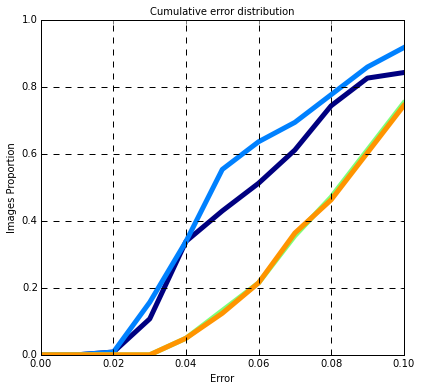
\includegraphics[width=0.48\columnwidth]{resources/DAAMBenchmark/face}
    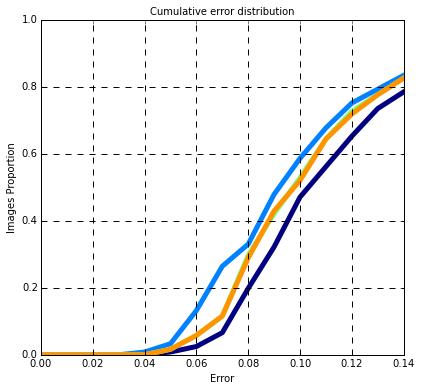
\includegraphics[width=0.48\columnwidth]{resources/DAAMBenchmark/ear}
    \caption{CEDs of faces and ears fitting performance for experiment \ref{exp:daam_benchmark}}
    \label{fig:daam_benchmark}
\end{figure}


\paragraph{Results} Cumulative Error Distribution (CED) curves for this experiment are shown in Figure \ref{fig:daam_benchmark}. We can readily observe that the accuracy achieved by ear models, in terms of the previous normalised point-to-point error measure, is lower than the one achieved by face models. This result is expected due to the more complex structure of the ear shape. Through visual inspection we determined that fitting errors below 0.1 for ears typically look plausible under the previous error measure where fitting errors below 0.6 for faces. Results show that, for this experiment, the fitting accuracy achieved by our dAAMs is marginally better to the one achieved by classic AAMs using intensity representations. In fact, classic AAM fail to improve the accuracy of the original initialisation on ears. Therefore the propose pipeline is capable of dealing with the complex structure of non-rigid shapes and learn dAAMs from simple curve line annotations that can compete and even surpass (in the case of a simple pixel intensity image representation) classic AAM, build from carefully annotated point landmarks, is quite remarkable.


\subsection{Arm Pose Estimation}
\label{exp:benchmark}


This experiment evaluates the localisation of arm joints using our skeleton prediction from outline fitting and compares it to state-of-the-art human pose estimation algorithms in-the-wild.
% We show here that training a patch-based AAM from our automatic outline annotations provides remarkable joints estimation.
In addition, the experiment investigates the impact of annotating outlines of human poses instead of annotating skeletons. Note that all results reported in this section were obtained by fitting patch-based AAM using the fast version of the Simultaneous Inverse Compositional algorithm (Fast-SIC) originally proposed by the authors of \cite{Papandreou2008}.



\paragraph{Dataset \& Error Metric} There exist several datasets for human pose estimation, with FLIC \cite{sapp2013modec}, BBC Pose \cite{pfister2015flowing}, Fashion Pose \cite{dantone2013human} and MPII \cite{andriluka14cvpr} being some of the most commonly-used ones. In this work, we report quantitative evaluation on BBC Pose, which contains the most consistent skeleton annotations among the relevant datasets.


The training of patch-based AAM for arms involves manual outline annotation from a combination of datasets, including H3D \cite{PoseletsICCV09}, Microsoft COCO \cite{lin2014microsoft}, MPII \cite{andriluka14cvpr}, Fashion Pose \cite{dantone2013human}, FLIC \cite{sapp2013modec} and BBC Poses \cite{pfister2015flowing}. The training set contains 891 training images from where 500 are annotated with outline manually. A dAAMs is built from 500 training images thereby produces dense correspondences for generating sparse outline annotation (29 landmarks). A patch-based AAM is build from sparse annotations before fitting to 391 images. Manual minor correction are required for putting those fitted image to training set. The final patch-based AAM is built from 891 images and validated on validation set given by BBC Pose.

In order to compare with current state-of-the-art human pose estimation on BBC Pose, we uses same error metric as BBC Poses does, which normalises testing images to have height of 256 pixels. Performance measure of experiments in this paper are plot with Cumulative Error Distribution (CED) curve, where graph shows accuracy against distance from ground truth in pixels on normalised images.


\begin{figure}[b!]
    \centering
    \includegraphics[width=\columnwidth]{resources/HandBenchmark/legend}
    \\
    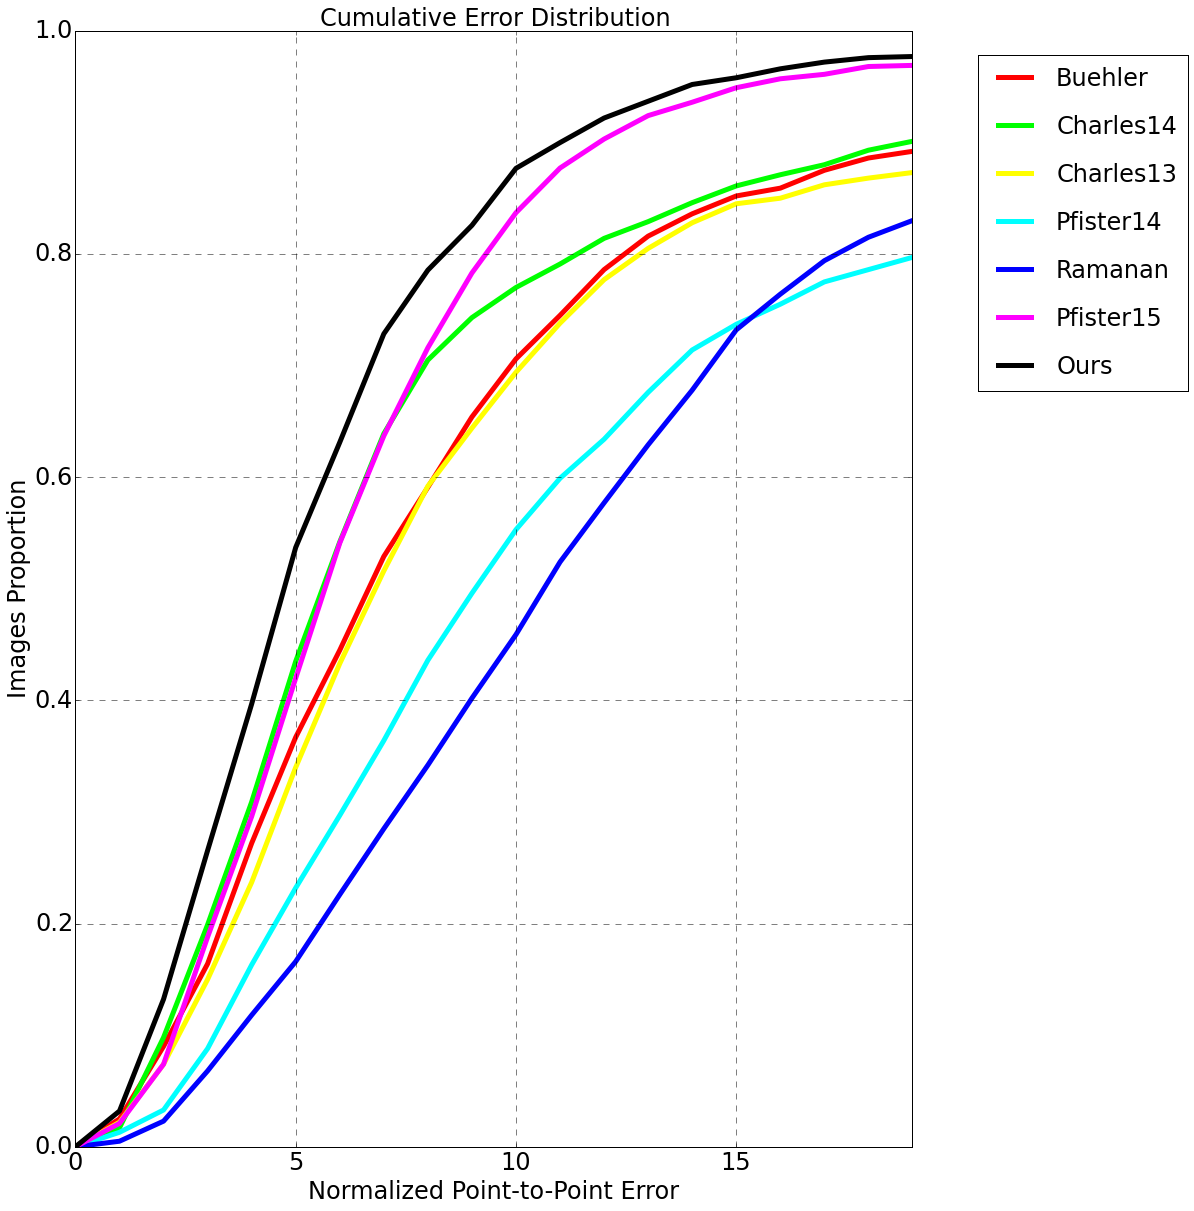
\includegraphics[width=0.48\columnwidth]{resources/HandBenchmark/wrist}
    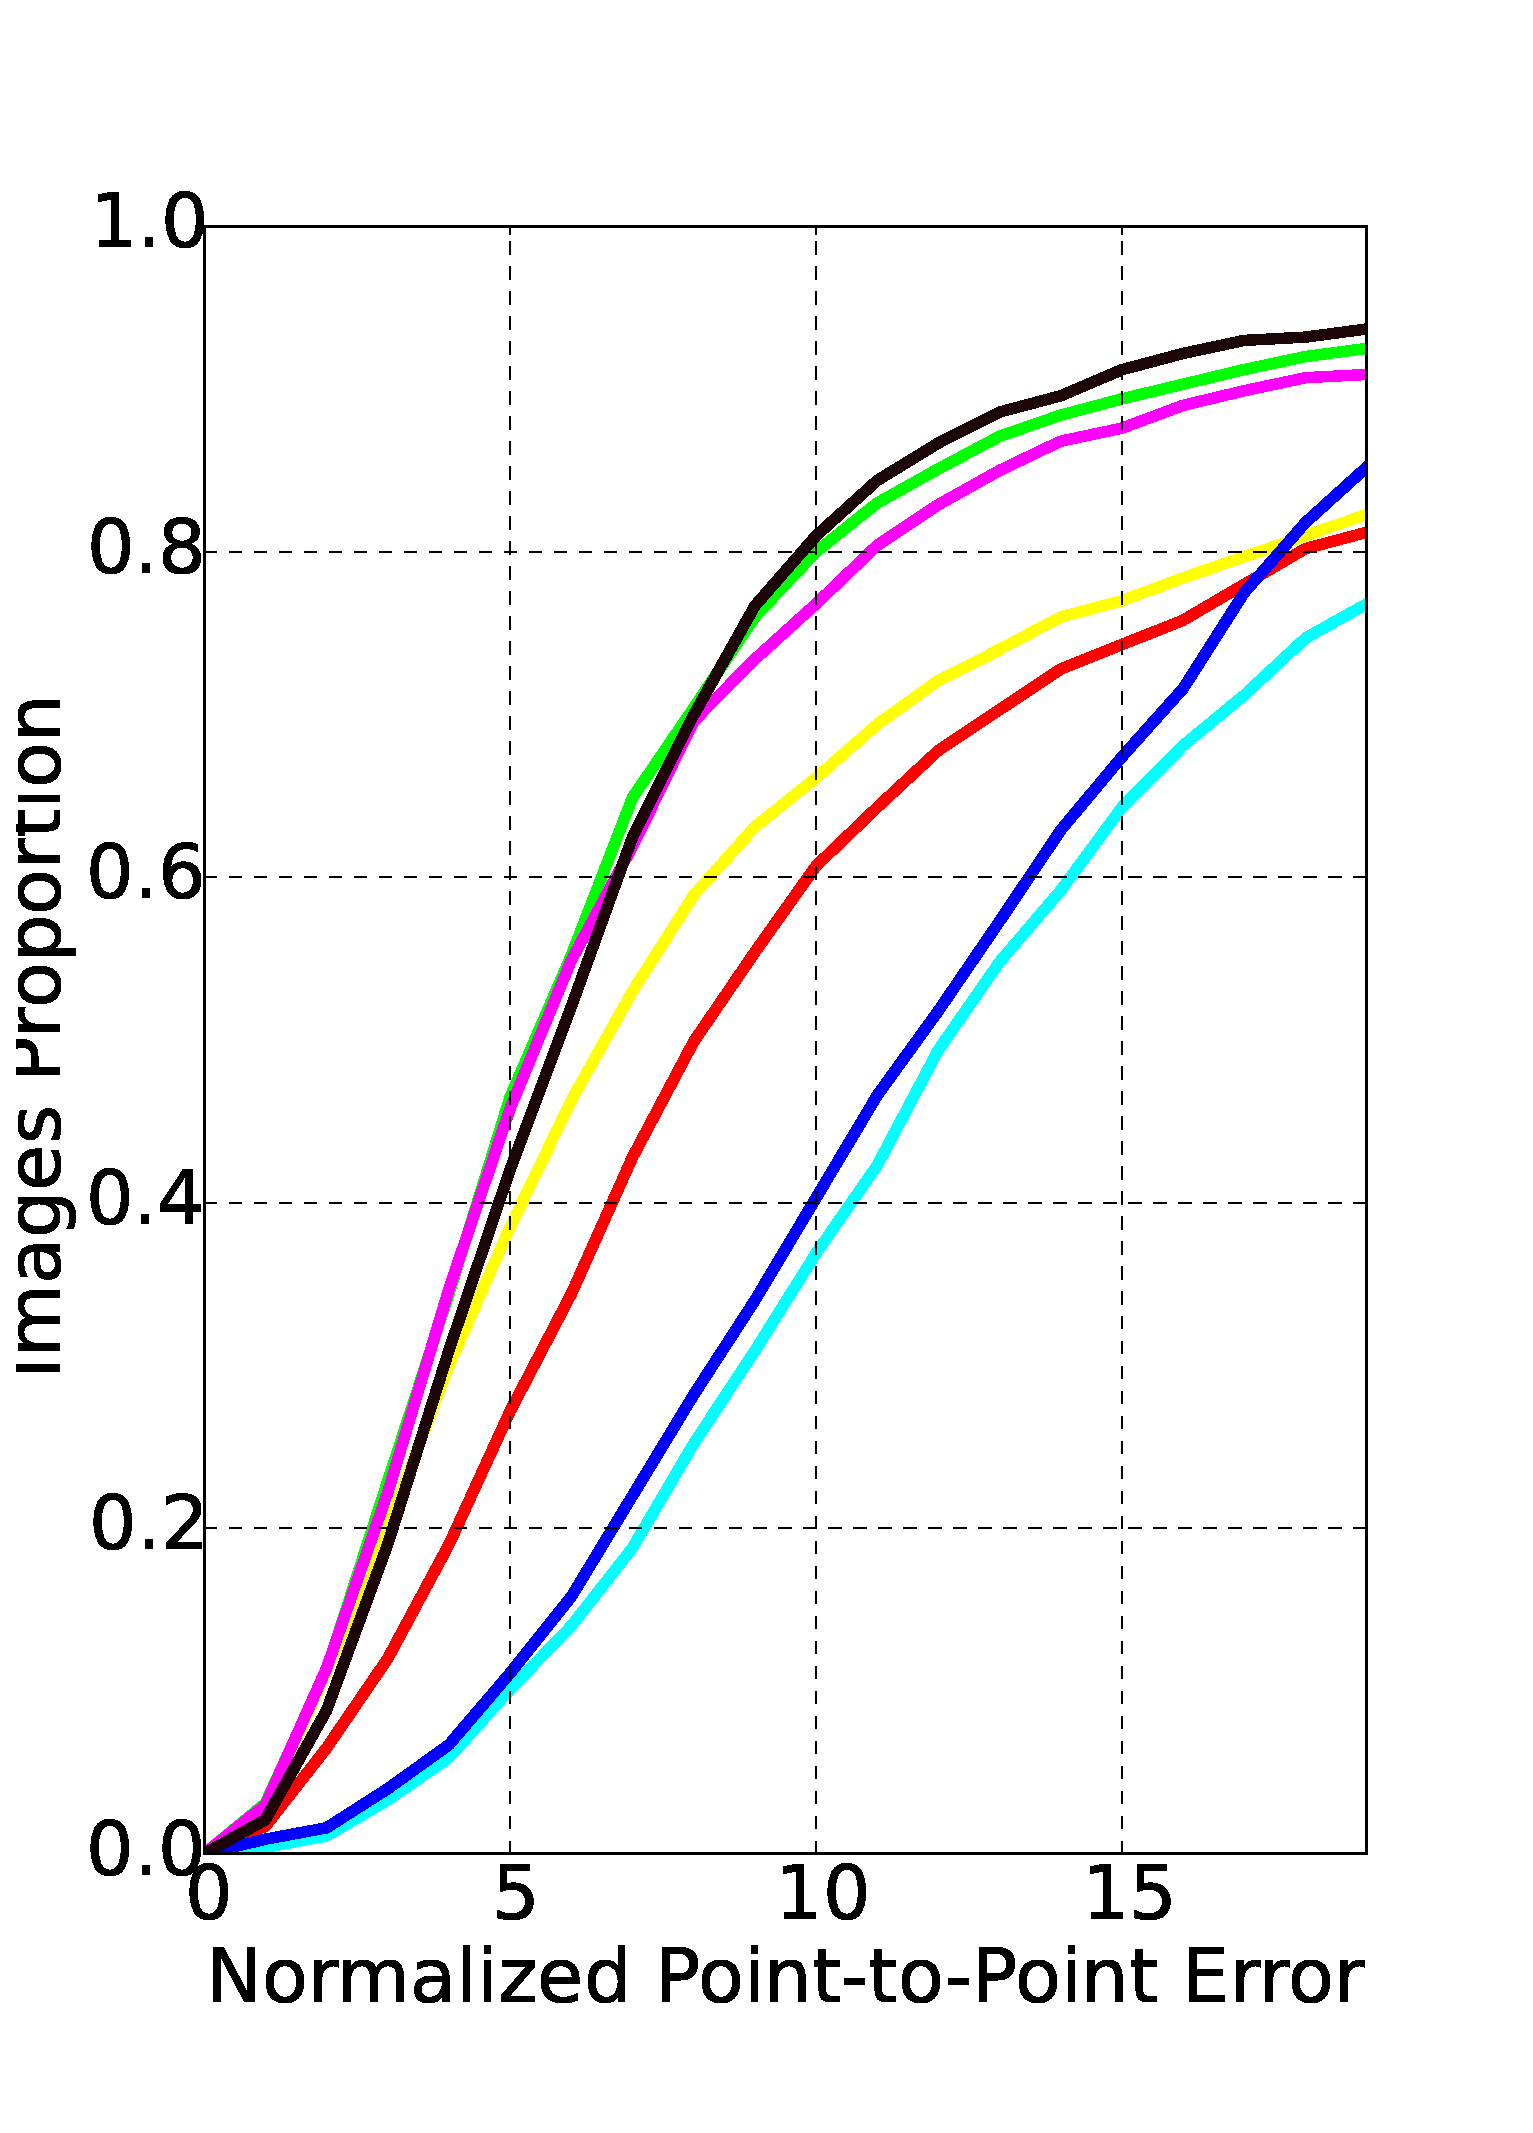
\includegraphics[width=0.48\columnwidth]{resources/HandBenchmark/elbow}
    \caption{CEDs over skeleton landmarks on BBC Pose database for experiment \ref{exp:benchmark}}
    \label{fig:hand_benchmark}
\end{figure}

\textbf{Experiments} Two experiments are undertaken in this section: 1) presenting training classic patch-based AAM from outline annotation provides remarkable joints estimation; 2) supporting outline annotation by comparing with training classic patch-based AAM from joint annotation.

First experiment presented the accuracy of predicting joints positions from establishing dense correspondences with outline fitting. We build patch-based AAM using 891 training hand images from a combination of datasets, where each image has 29 landmarks annotated alone its boundary. SIFT \cite{PoseletsICCV09} feature is used from image representation for our model. Model fitting is initialised based on current state-of-the-art human pose estimation algorithms (including Buehler \cite{buehler2011upper}, Charles14 \cite{charles2014upper}, Charles13 \cite{charles2013domain}, Pfister14 \cite{pfister2015deep}, Ramanan \cite{yang2013articulated} and Pfister15 \cite{pfister2015flowing}) on BBC Pose \cite{pfister2015flowing} dataset. Results for this experiment are reported over 1000 testing images BBC Pose Provided, which human upper-body pose are landmark with 7 points on skeleton. For our model, joints are projected from the dense correspondence generated from our proposed method.

Second experiment investigates the disadvantages of using skeleton annotation. We build patch-based AAM on joints with same training data and with SIFT representation. Both models are fine-tuned on BBC Pose validation set. The fitting procedure is performed under exactly same condition, e.g. same testing set and initialisation position.

CED Curves for both experiments are shown in Figure \ref{fig:hand_benchmark} while fitting statistics are shown in supplementary material. Results show that, for first experiment, the fitting accuracy achieved by our method outperformed current state-of-the-art algorithms. In particular, our method improves performance of current best method \cite{pfister2015flowing} by a notable amount (9\% with error less than 6pt) on wrist, as well as marginal improvement on elbow estimation. While for second experiment, patch-based AAM trained with outline significantly outperforms path AAM trained with joints as we expected. Note that path AMM trained with Joints still comparable even marginally better than recent algorithms.




% \begin{table}[b!]
%     \small
%     \centering
%     \begin{tabular}{|l|c|c|c||c|c|c|}
%         \hline
%                             & \multicolumn{3}{c||}{Wrist} & \multicolumn{3}{c|}{Elbow}\\
%         \hline
%         \emph{Method}       & \emph{mean} & \emph{std} & $\leq 6pt$ & \emph{mean} & \emph{std} & $\leq 6pt$\\
%         \hline\hline
%         Buehler             & 12.08    & 19.94        & 44.5\%       & 12.94    & 14.65        & 34.4\%\\
%         Charles14           & 11.81    & 20.89        & 54.2\%       &  8.30    & 11.00        & \textbf{55.2\%}\\
%         Charles13           & 13.78    & 22.39        & 43.3\%       & 13.17    & 18.74        & 46.3\%\\
%         Pfister14           & 14.69    & 17.89        & 29.7\%       & 14.60    & 10.59        & 14.0\%\\
%         Ramanan             & 15.59    & 19.04        & 22.6\%       & 15.53    & 10.82        & 15.8\%\\
%         Pfister15           & 7.62     & 11.04        & 54.1\%       &  8.84    & 11.44        & 54.9\%\\
%         \hline\hline
%         Ours                & \textbf{6.71}& \textbf{10.90}   & \textbf{63.1\%}       & \textbf{8.20}     &  \textbf{10.54}        & 52.1\%\\
%         \hline
%     \end{tabular}
%     \caption{Fitting statistics on BBC Pose database for experiment \ref{exp:benchmark}}
%     \label{tab:hand_benchmark}
% \end{table}

\begin{figure*}[!t]
    \newcommand{\fh}{0.24\columnwidth}
    \centering
    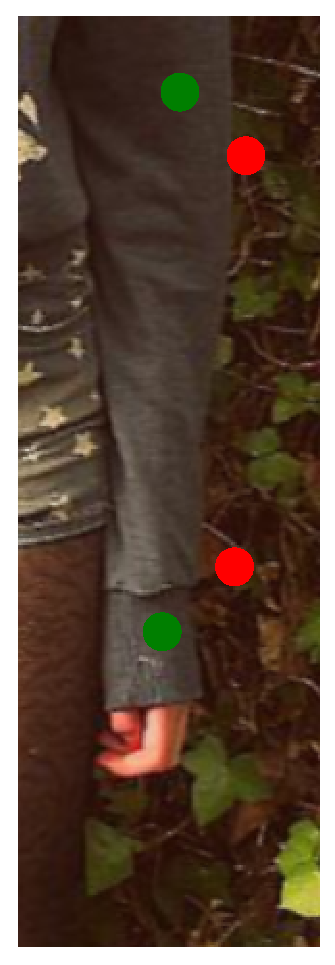
\includegraphics[height=\fh]{resources/Fixing/fix_1}
    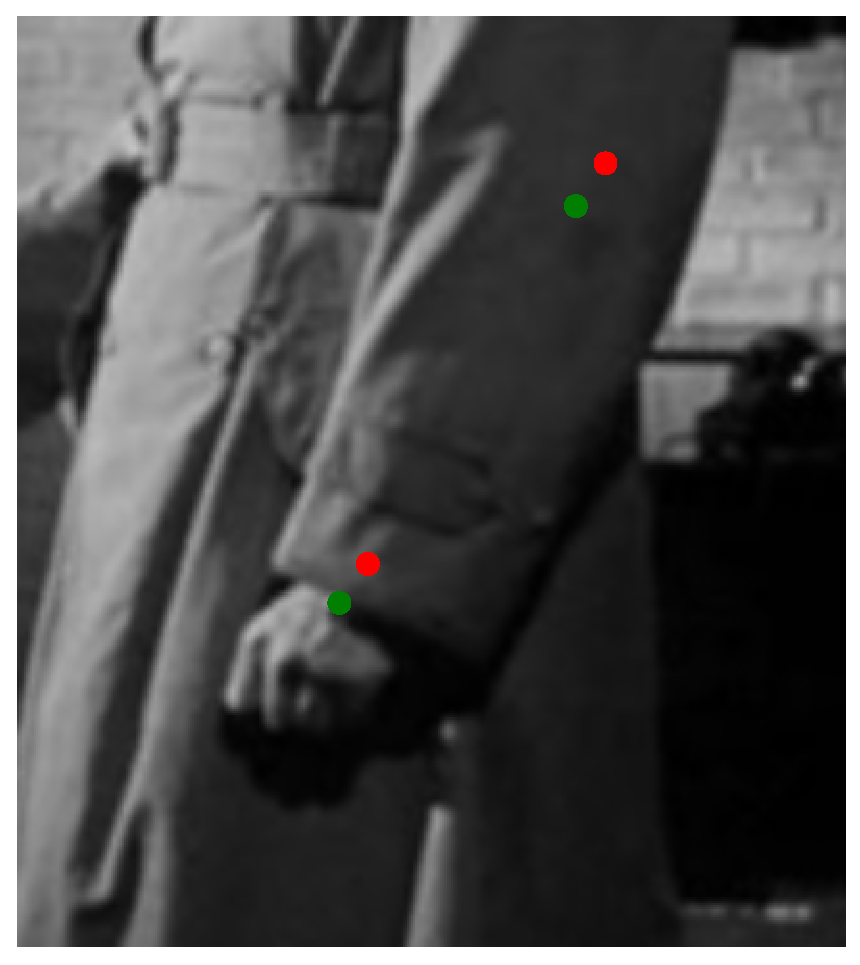
\includegraphics[height=\fh]{resources/Fixing/fix_2}
    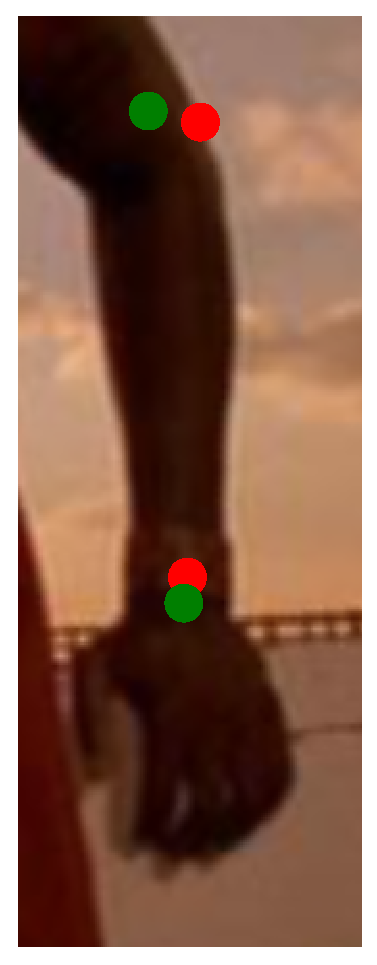
\includegraphics[height=\fh]{resources/Fixing/fix_3}
    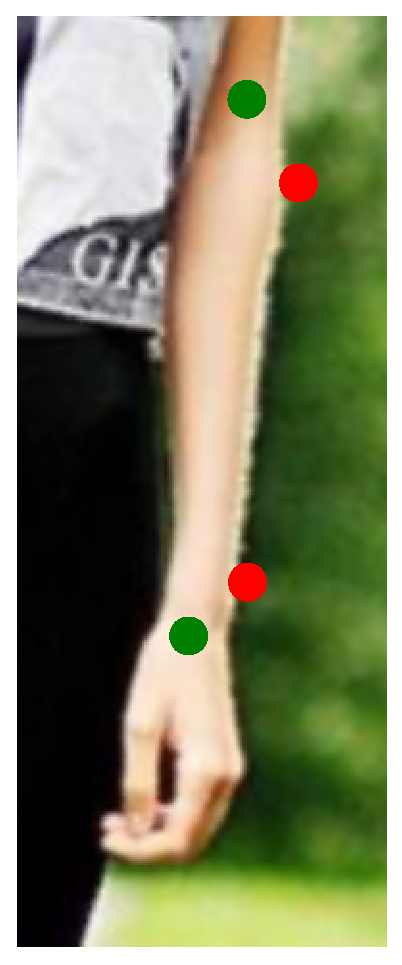
\includegraphics[height=\fh]{resources/Fixing/fix_5}
    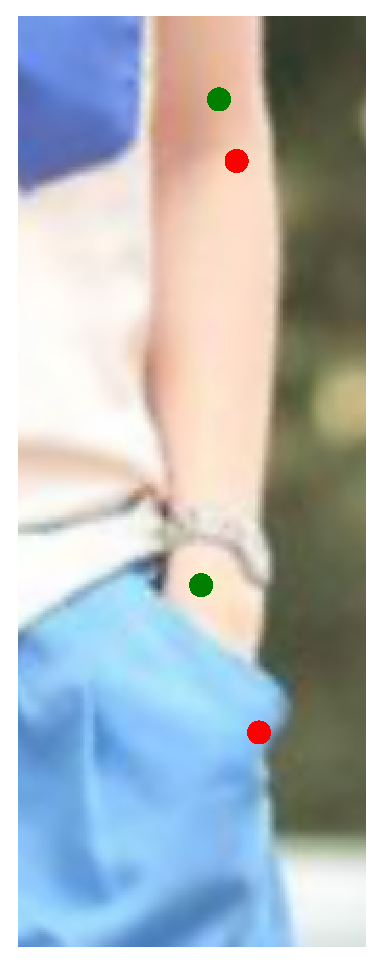
\includegraphics[height=\fh]{resources/Fixing/fix_6}
    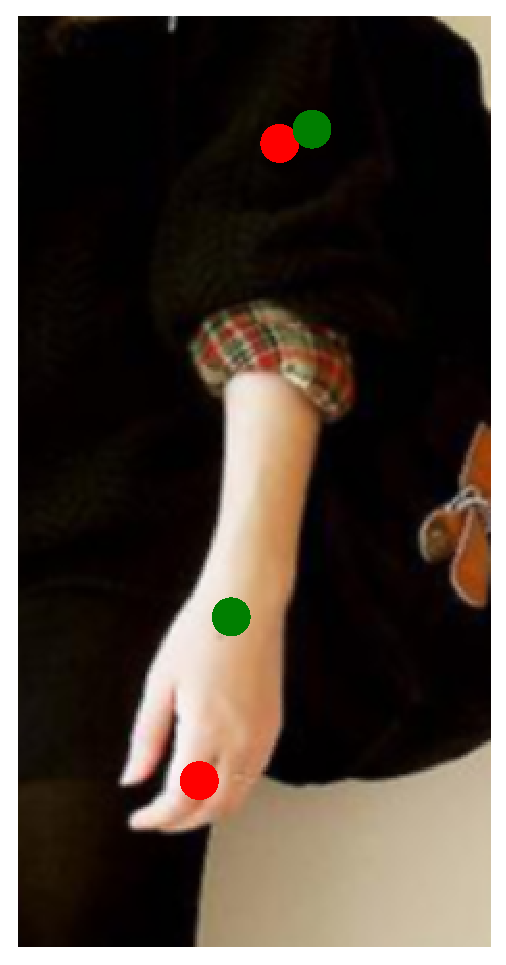
\includegraphics[height=\fh]{resources/Fixing/fix_7}
    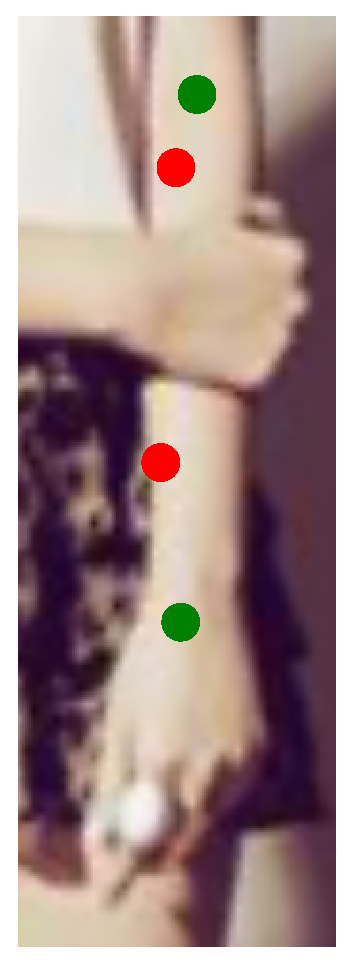
\includegraphics[height=\fh]{resources/Fixing/fix_8}
    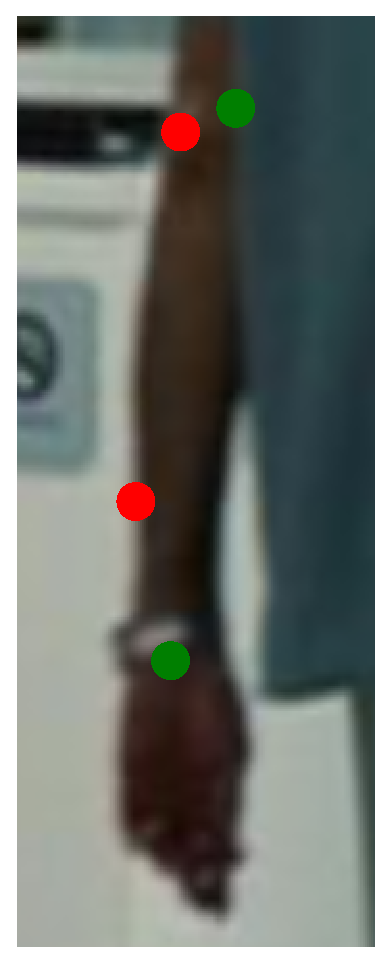
\includegraphics[height=\fh]{resources/Fixing/fix_9}
    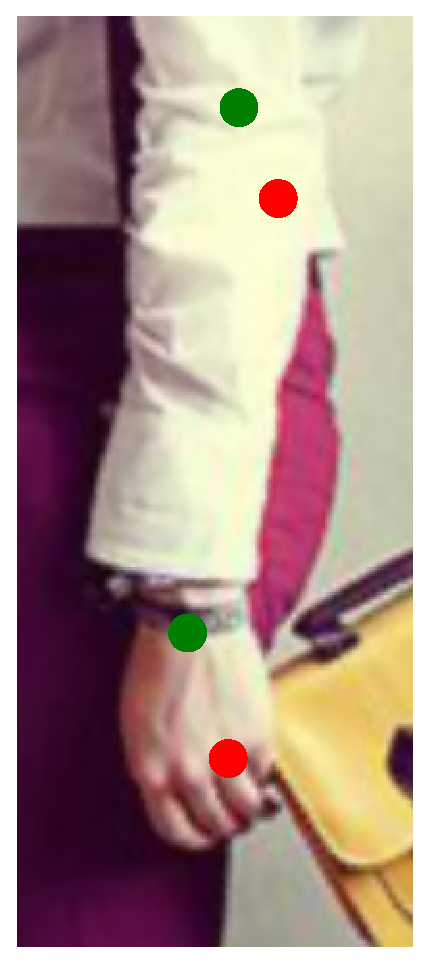
\includegraphics[height=\fh]{resources/Fixing/fix_10}
    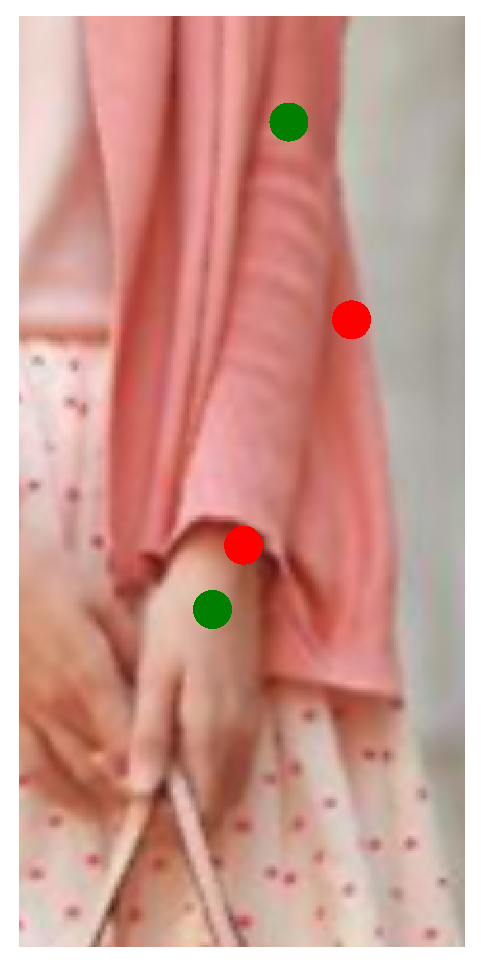
\includegraphics[height=\fh]{resources/Fixing/fix_20}
    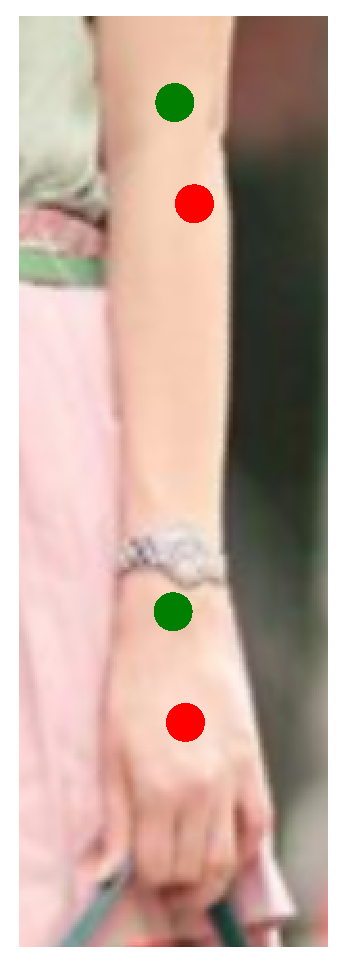
\includegraphics[height=\fh]{resources/Fixing/fix_12}
    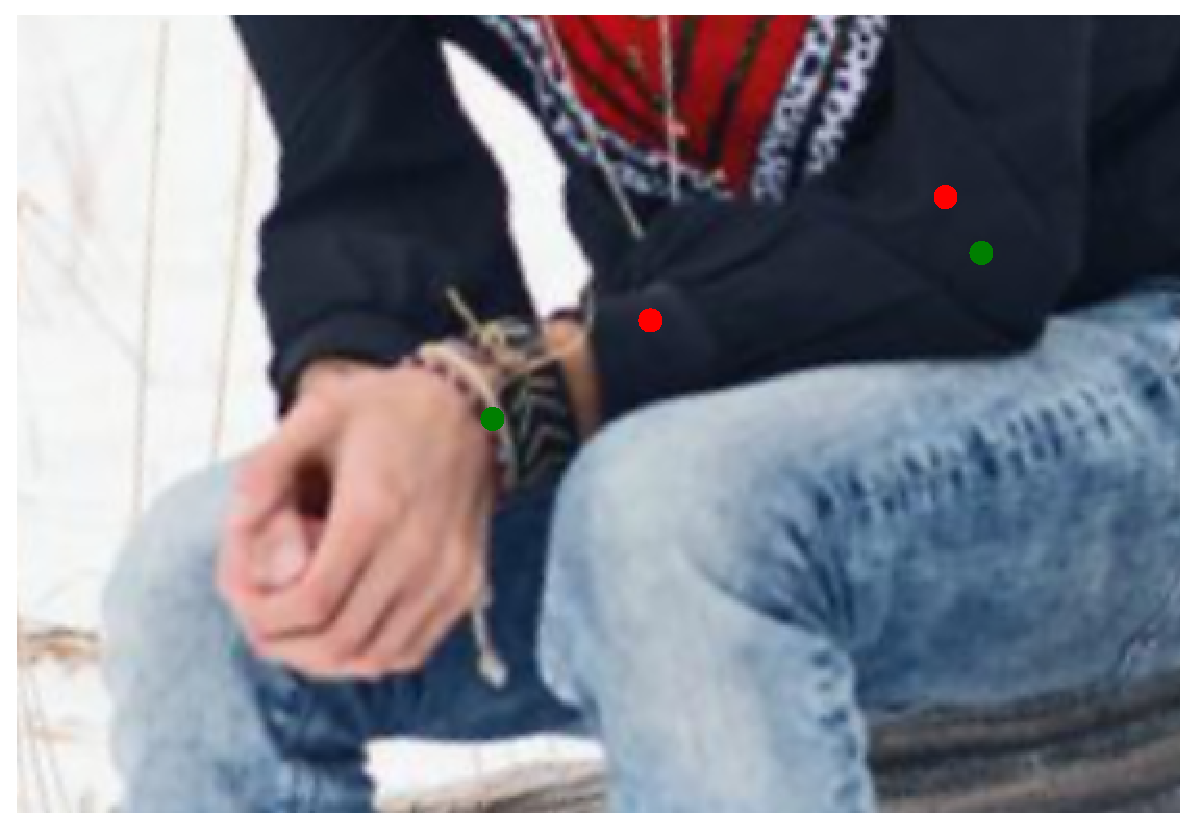
\includegraphics[height=\fh]{resources/Fixing/fix_13}
    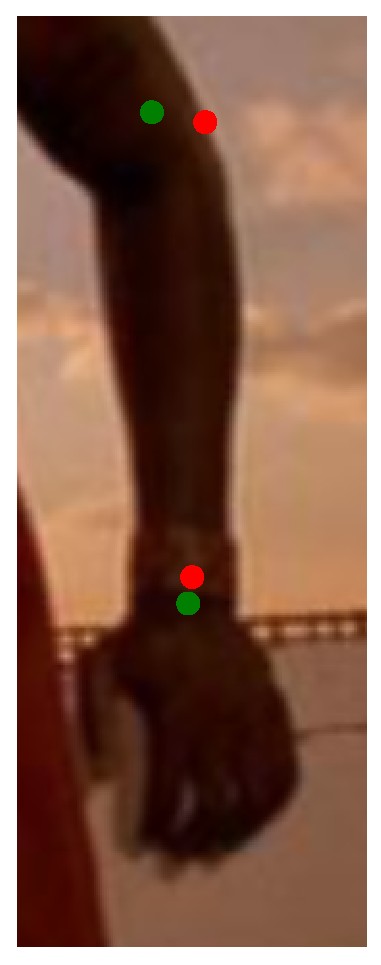
\includegraphics[height=\fh]{resources/Fixing/fix_14}
    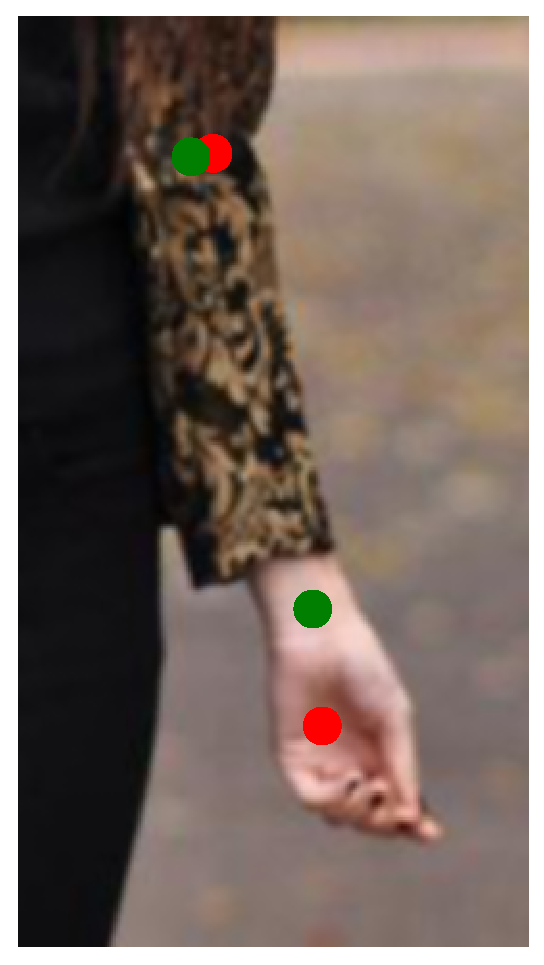
\includegraphics[height=\fh]{resources/Fixing/fix_15}
    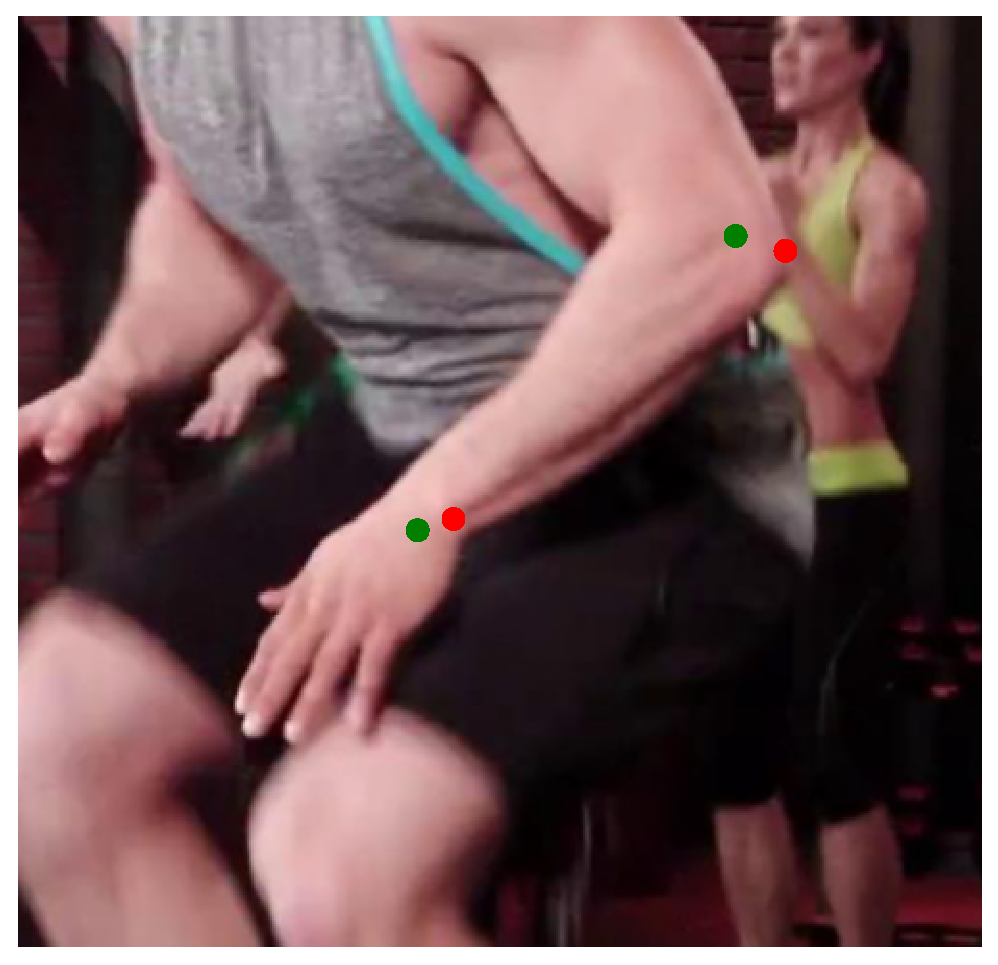
\includegraphics[height=\fh]{resources/Fixing/fix_17}
    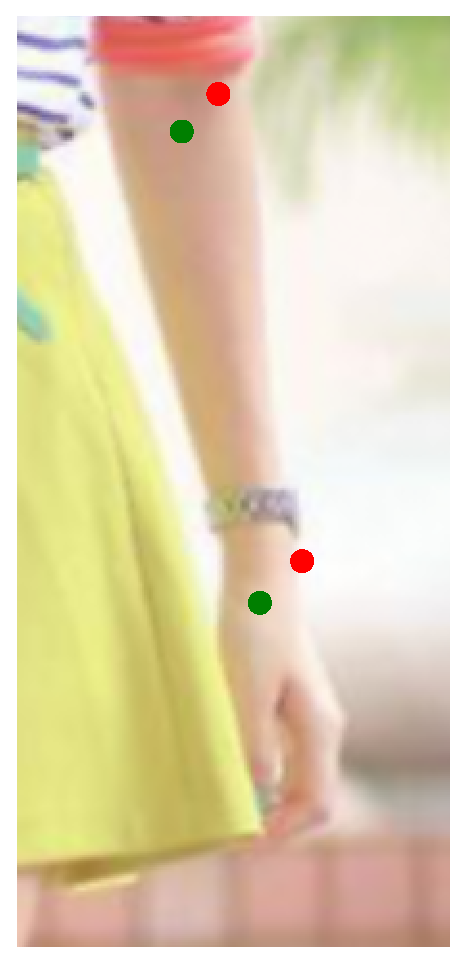
\includegraphics[height=\fh]{resources/Fixing/fix_18}
    % 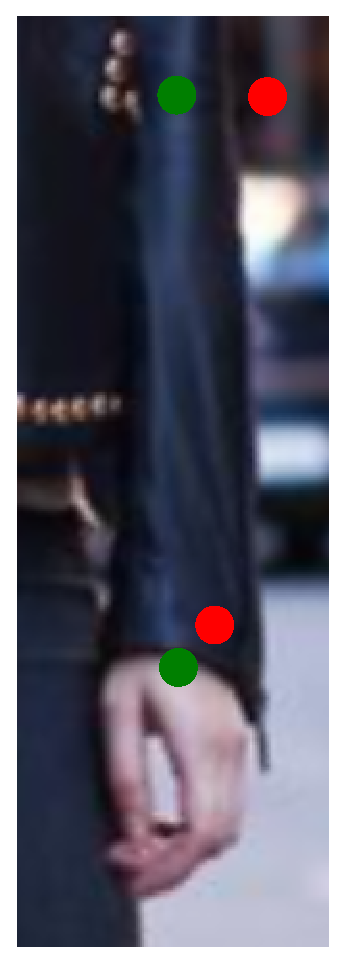
\includegraphics[height=\fh]{resources/Fixing/fix_19}
    \caption{Demonstration of annotation correction using our method for experiment \ref{exp:qualitative}. \emph{Red} dots refer to officially provided landmarks, and \emph{green} dots are corrected position.}
    \label{fig:qualitative}
\end{figure*}

\begin{figure*}[!t]
    \newcommand{\ofh}{0.24\columnwidth}
    \centering
    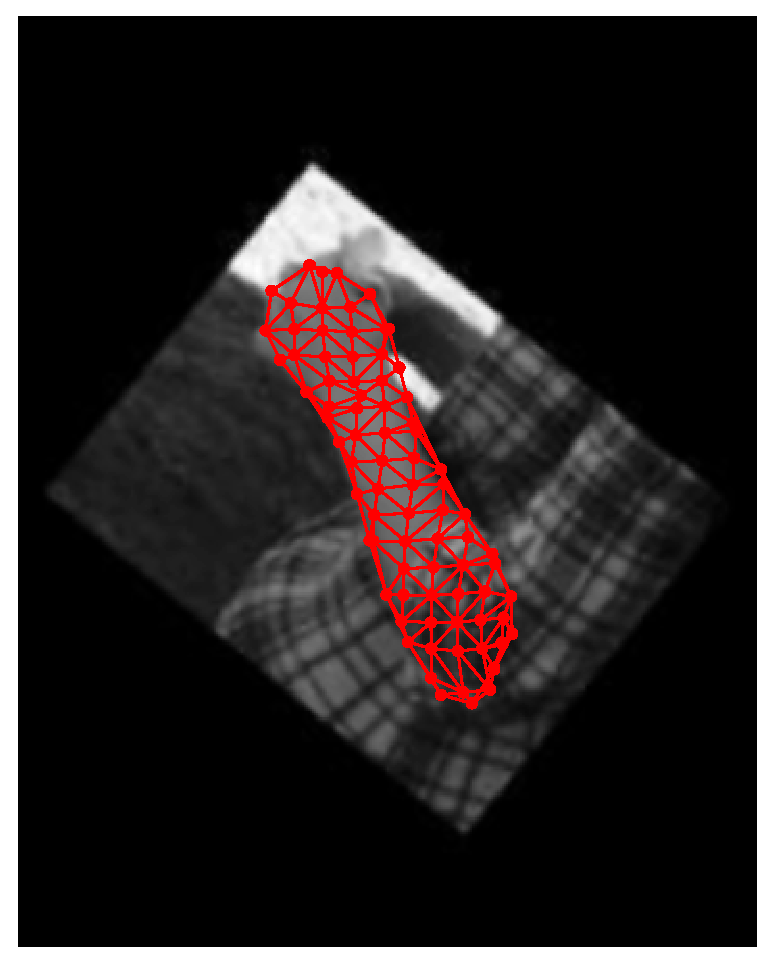
\includegraphics[height=\ofh]{resources/Fittings/20.eps}
    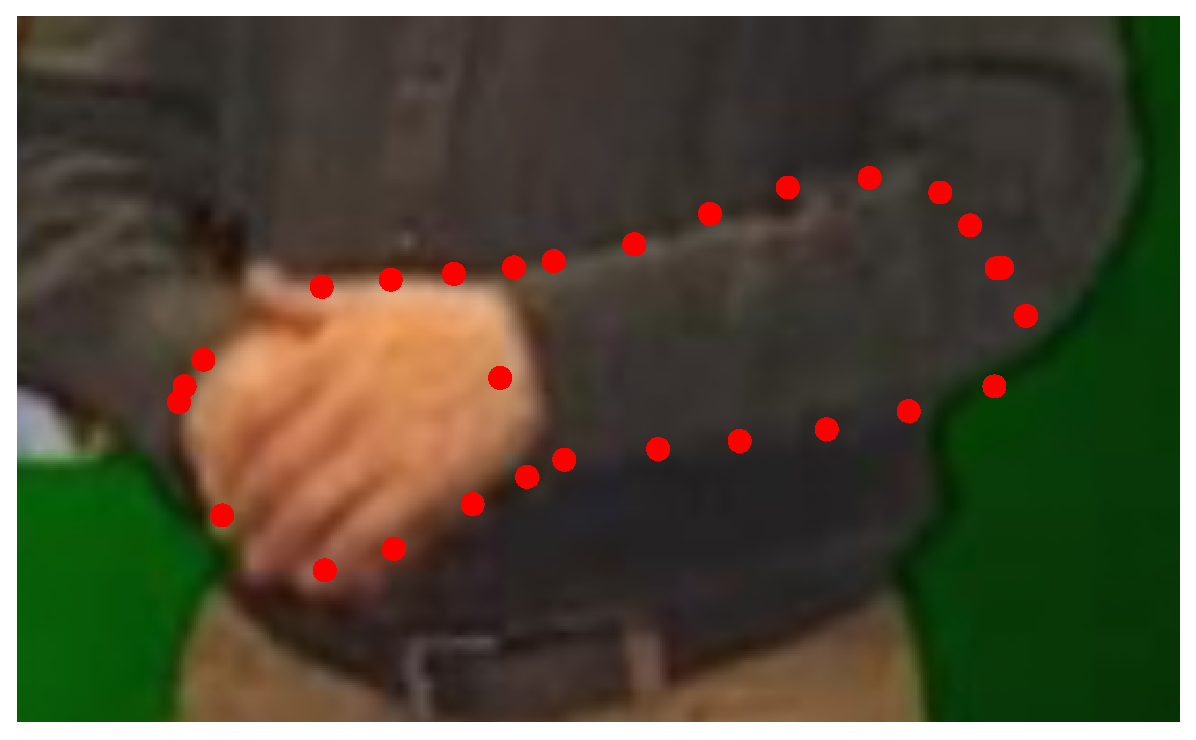
\includegraphics[height=\ofh]{resources/Fittings/3.eps}
    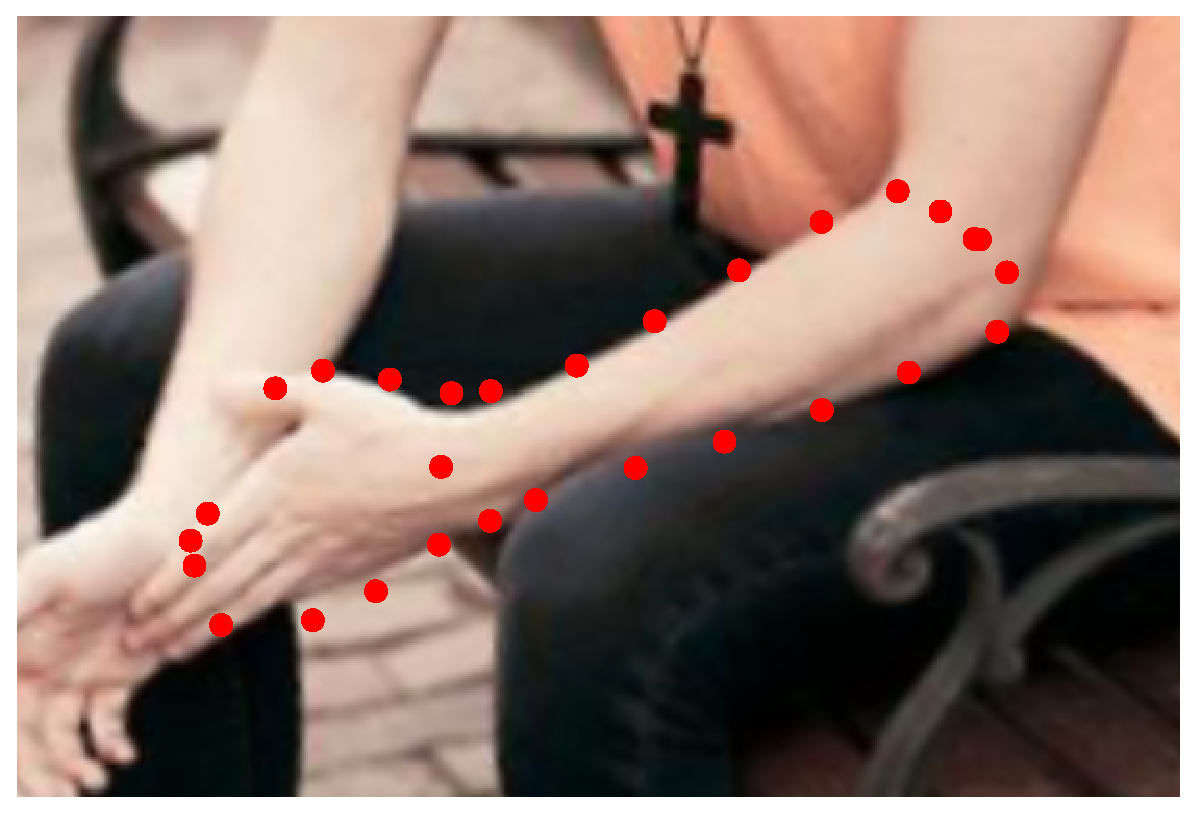
\includegraphics[height=\ofh]{resources/Fittings/19.eps}
    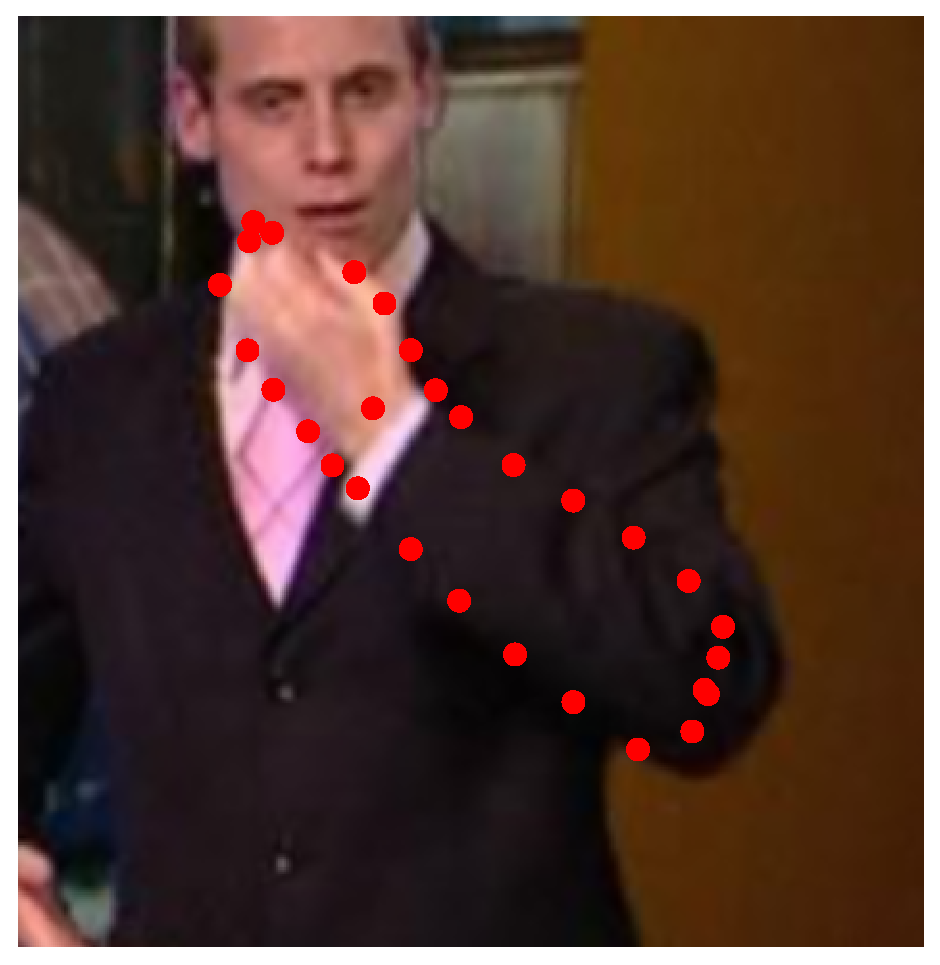
\includegraphics[height=\ofh]{resources/Fittings/4.eps}
    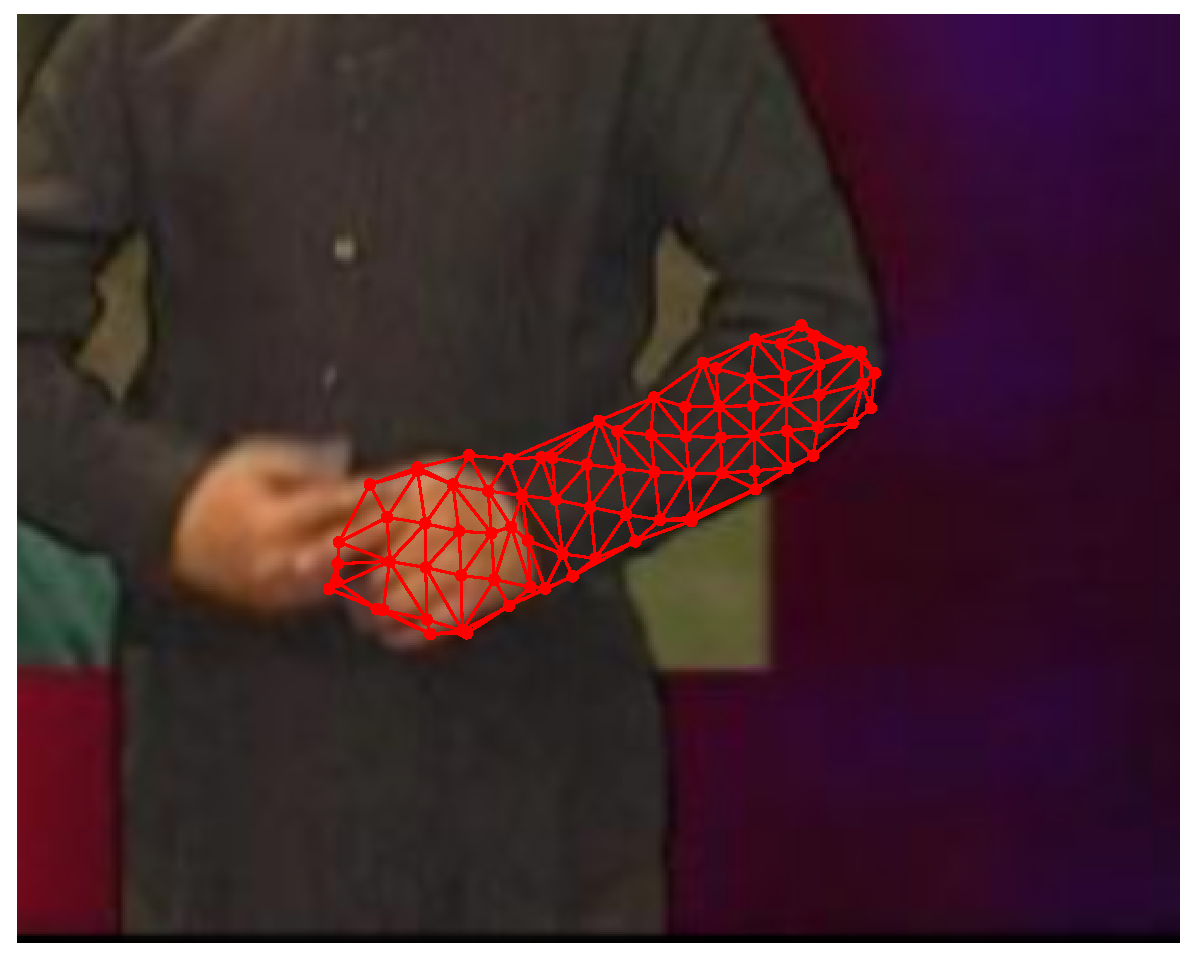
\includegraphics[height=\ofh]{resources/Fittings/6.eps}
    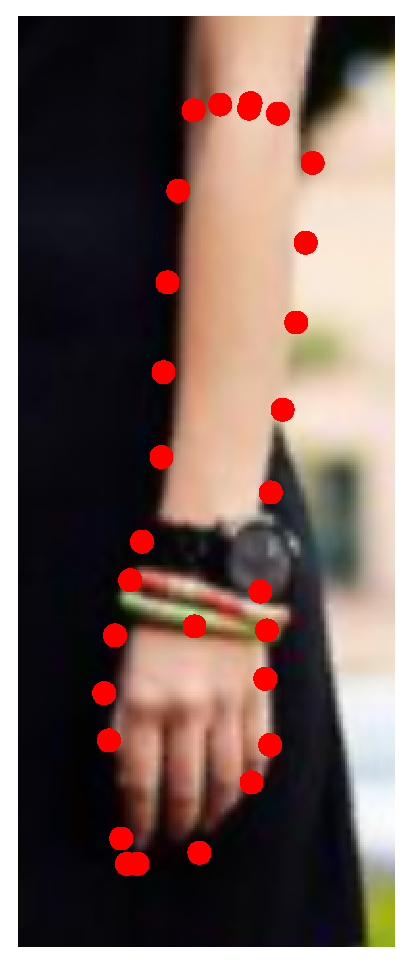
\includegraphics[height=\ofh]{resources/Fittings/15.eps}
    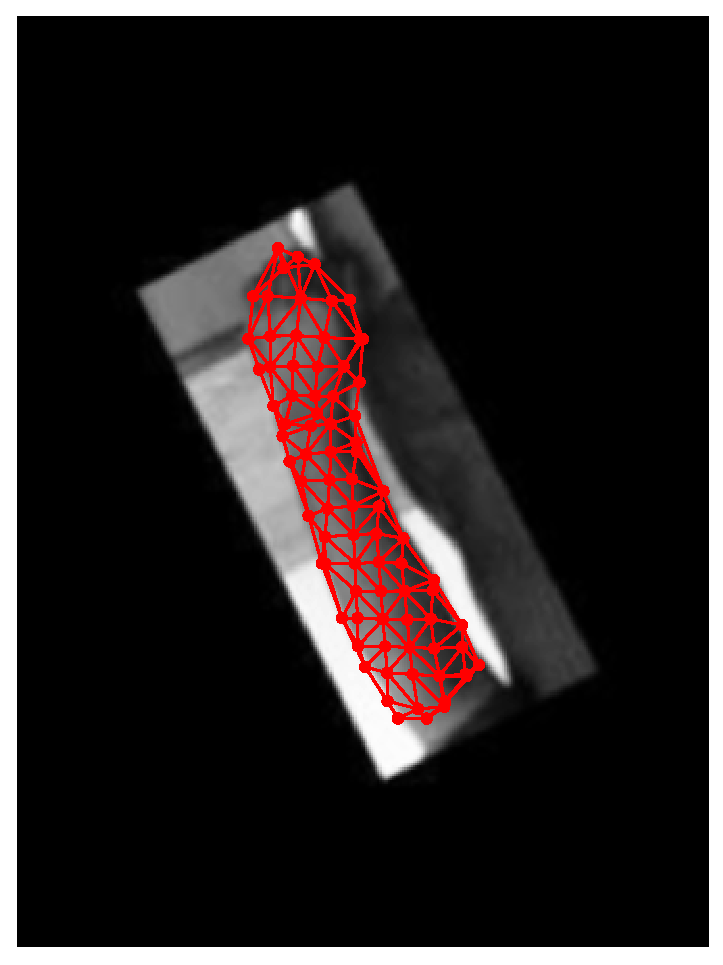
\includegraphics[height=\ofh]{resources/Fittings/7.eps}
    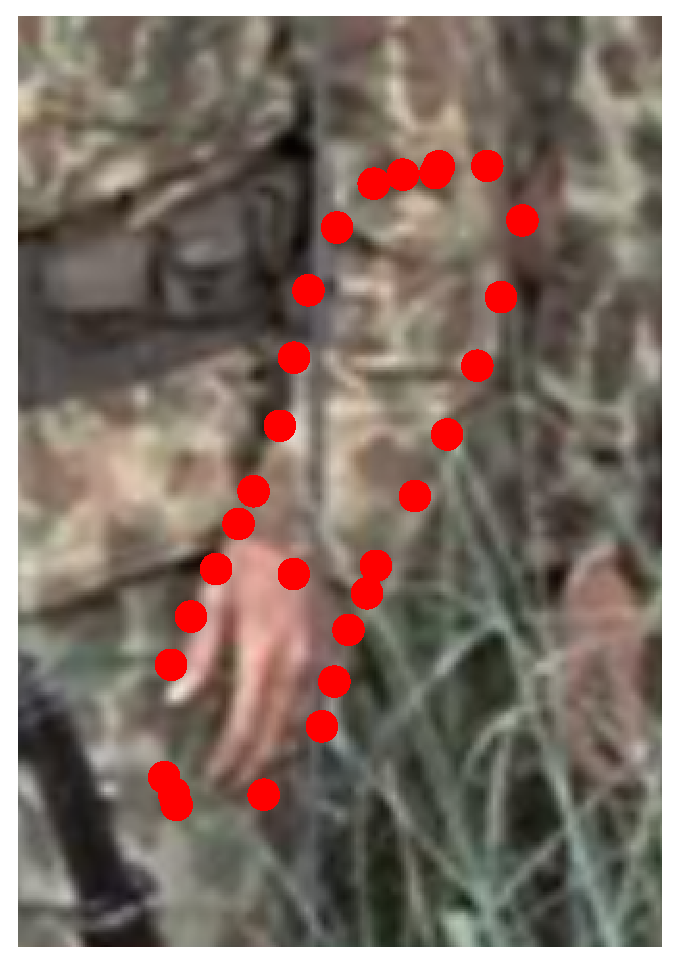
\includegraphics[height=\ofh]{resources/Fittings/8.eps}
    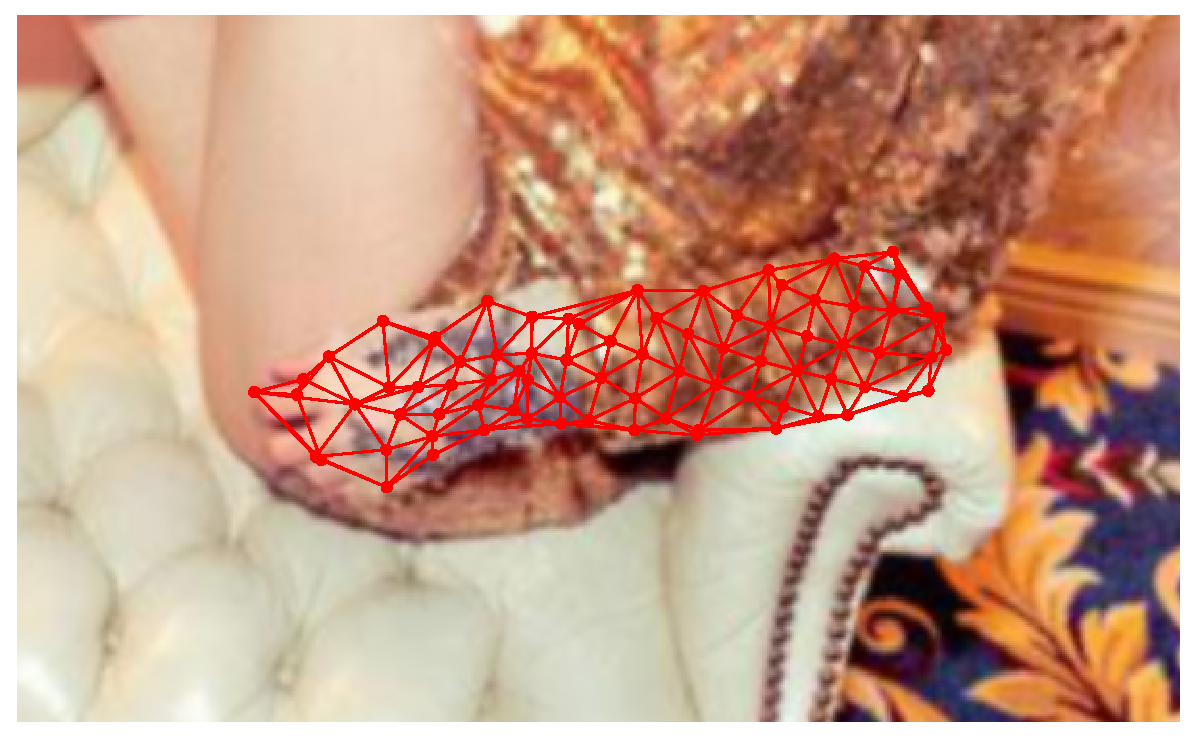
\includegraphics[height=\ofh]{resources/Fittings/13.eps}
    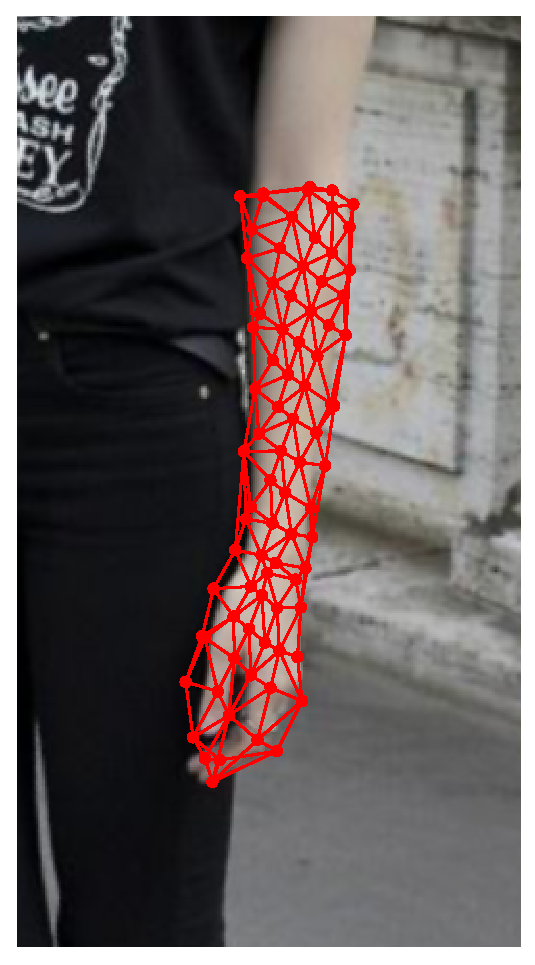
\includegraphics[height=\ofh]{resources/Fittings/17.eps}
    \\
    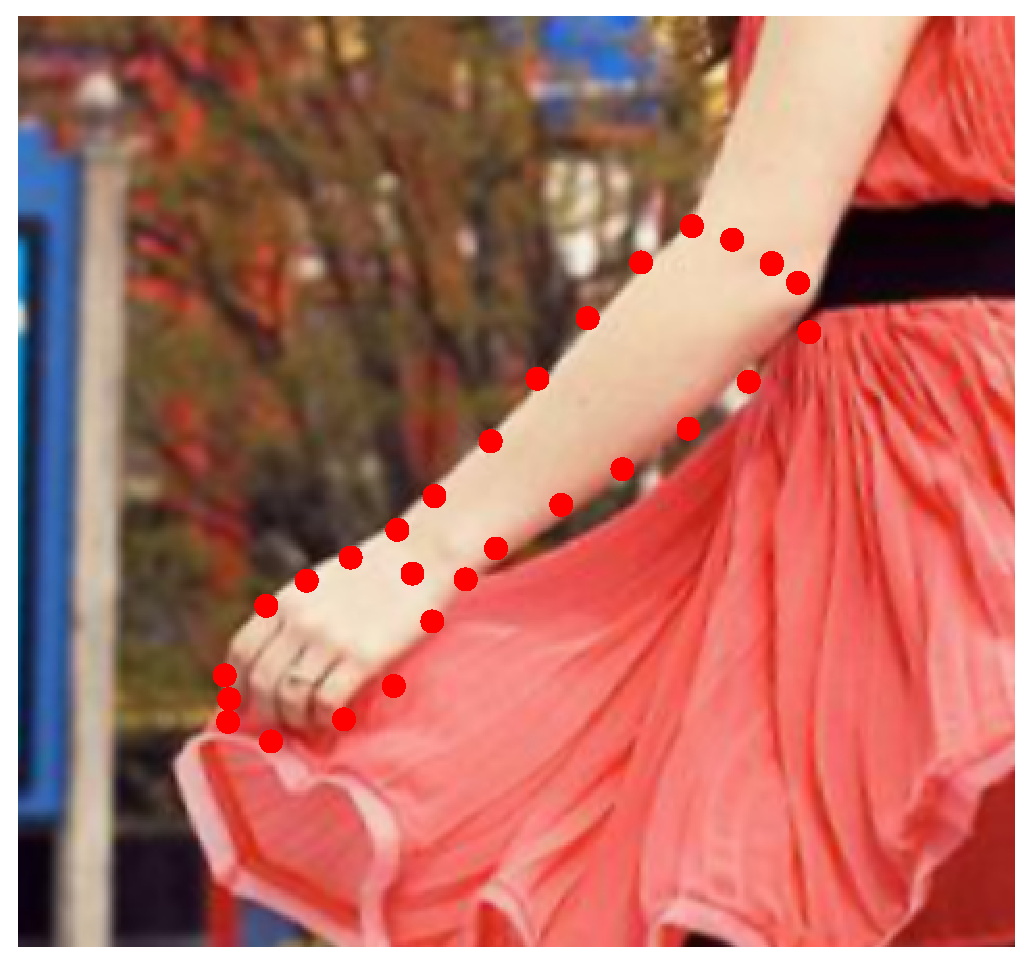
\includegraphics[height=\ofh]{resources/Fittings/21.eps}
    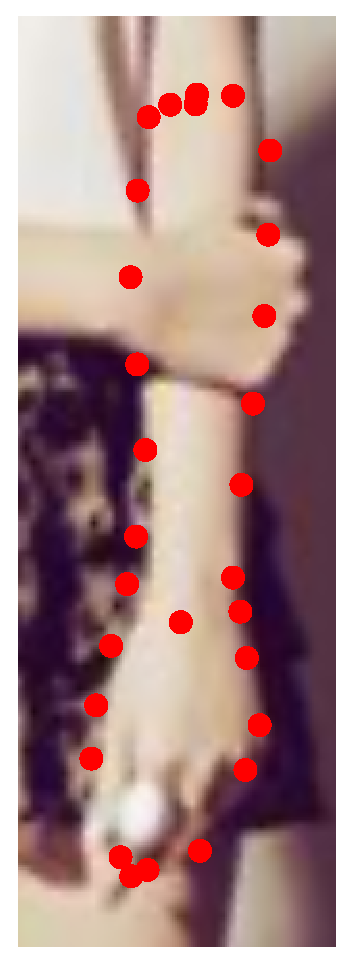
\includegraphics[height=\ofh]{resources/Fittings/23.eps}
    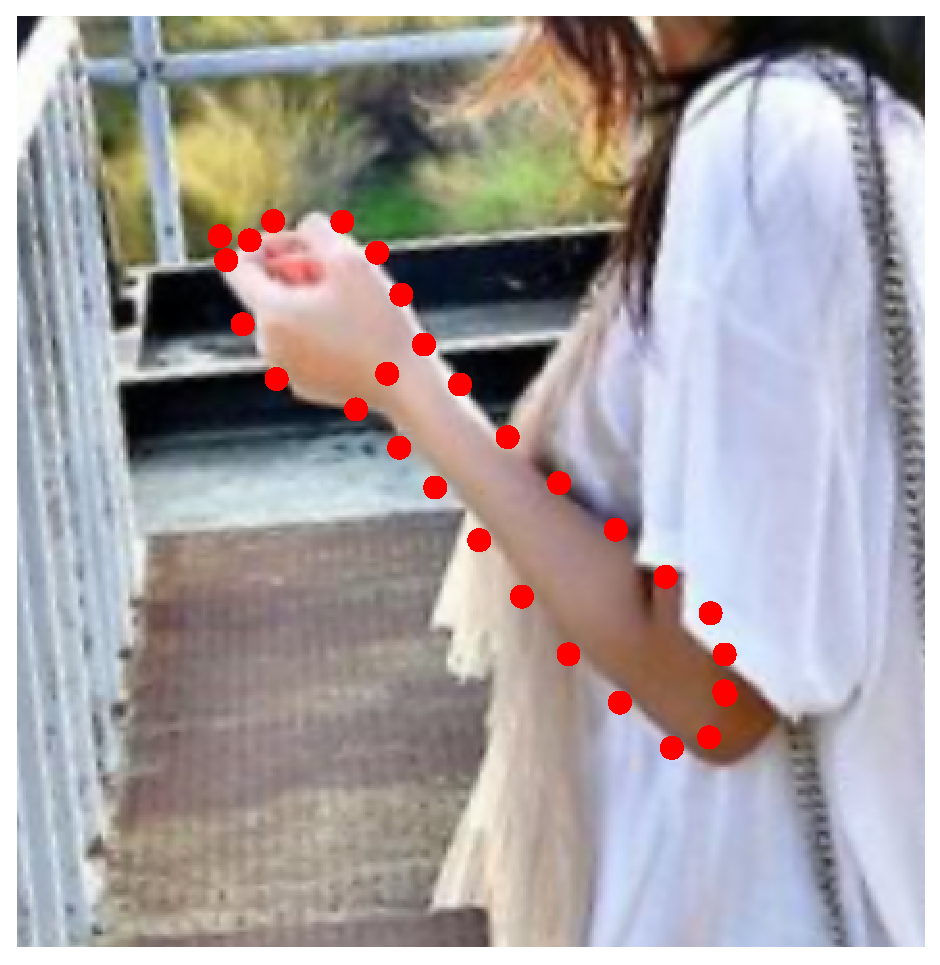
\includegraphics[height=\ofh]{resources/Fittings/25.eps}
    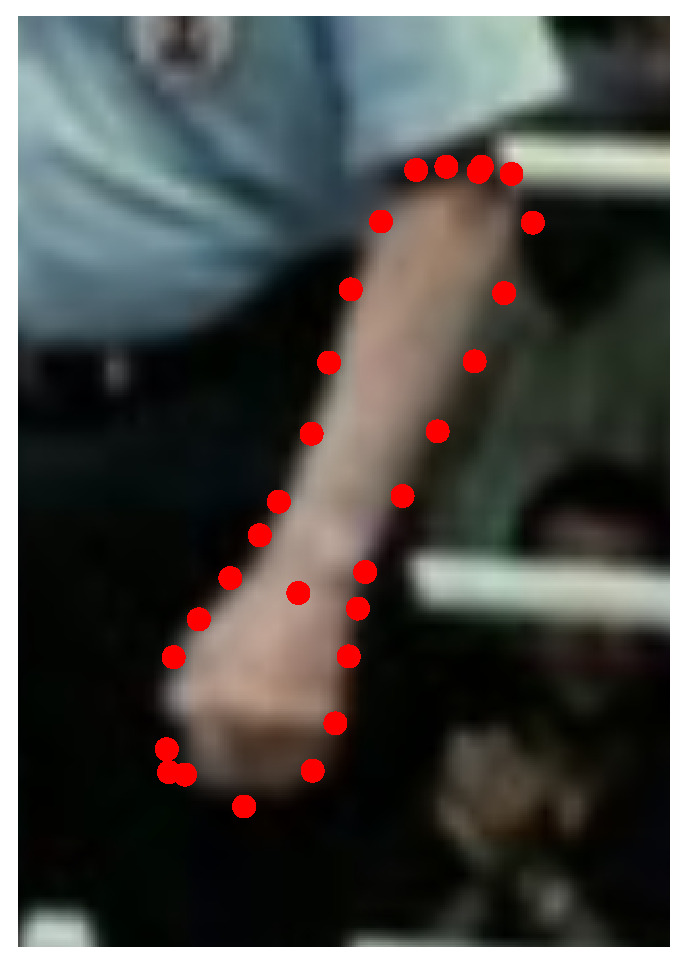
\includegraphics[height=\ofh]{resources/Fittings/27.eps}
    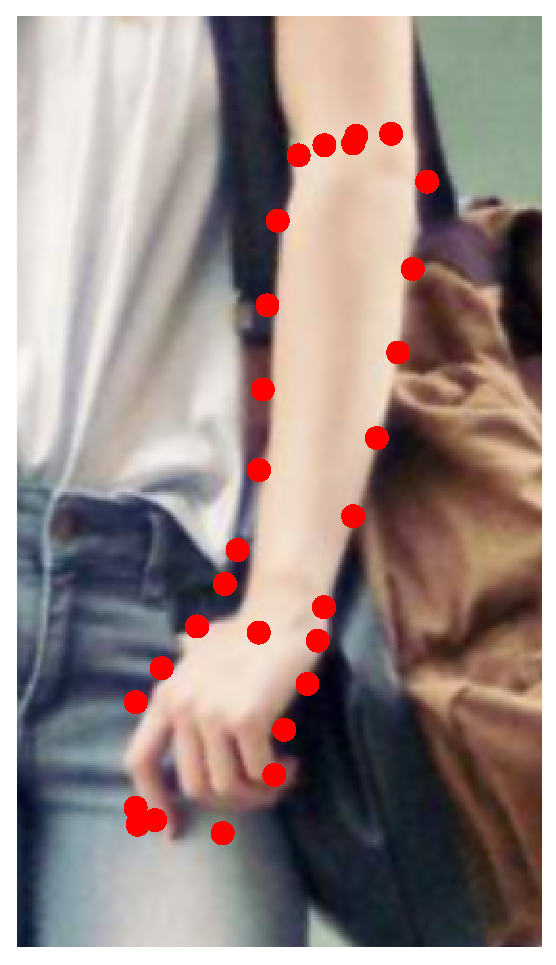
\includegraphics[height=\ofh]{resources/Fittings/29.eps}
    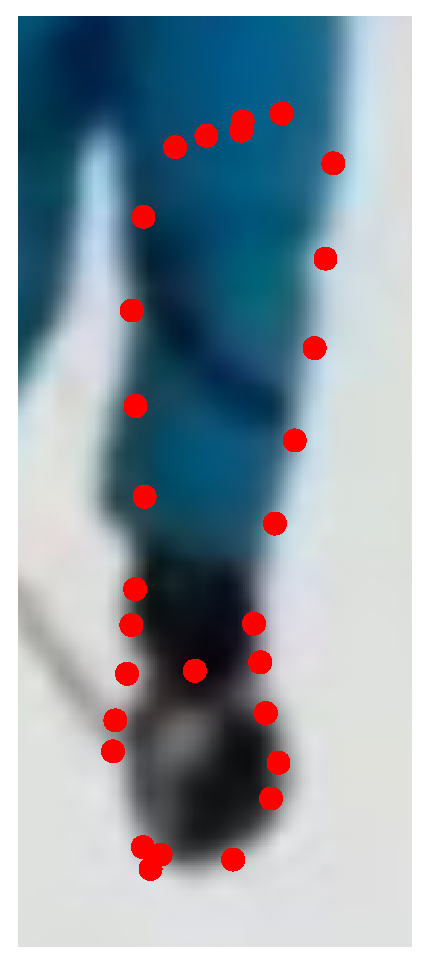
\includegraphics[height=\ofh]{resources/Fittings/31.eps}
    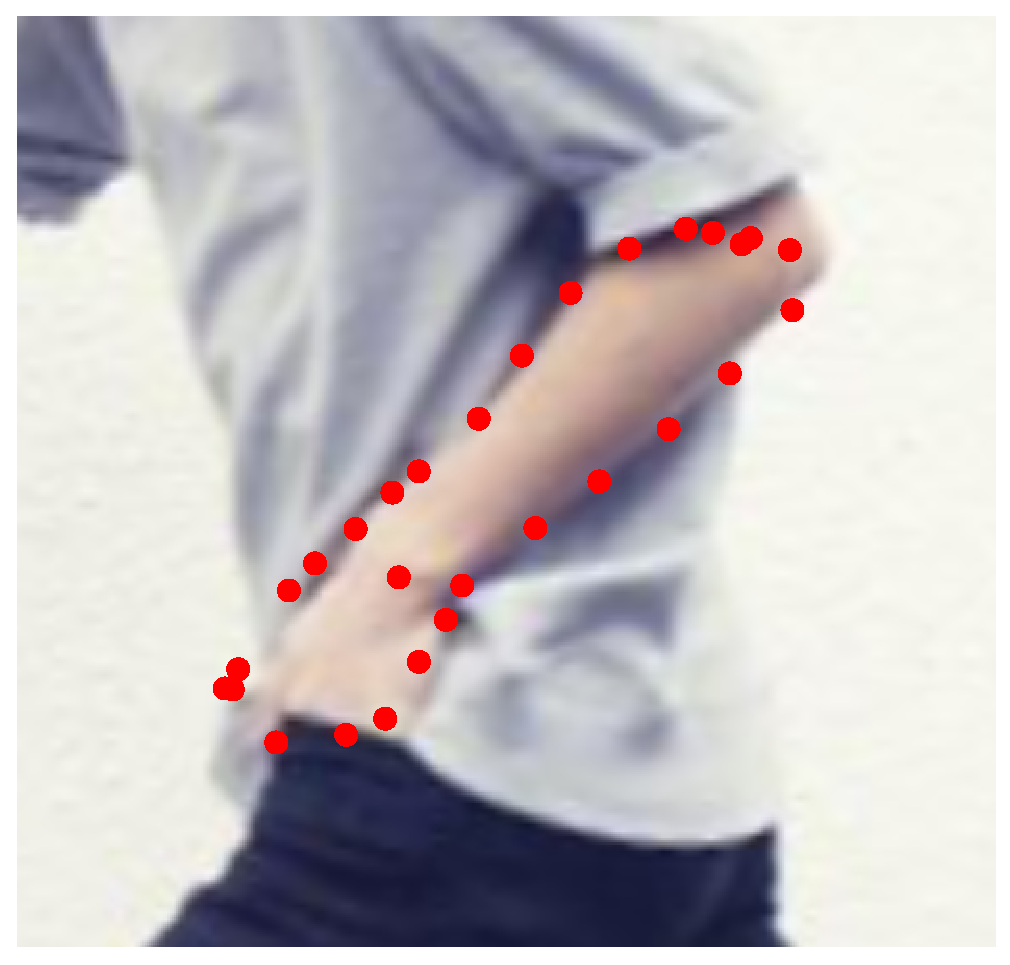
\includegraphics[height=\ofh]{resources/Fittings/33.eps}
    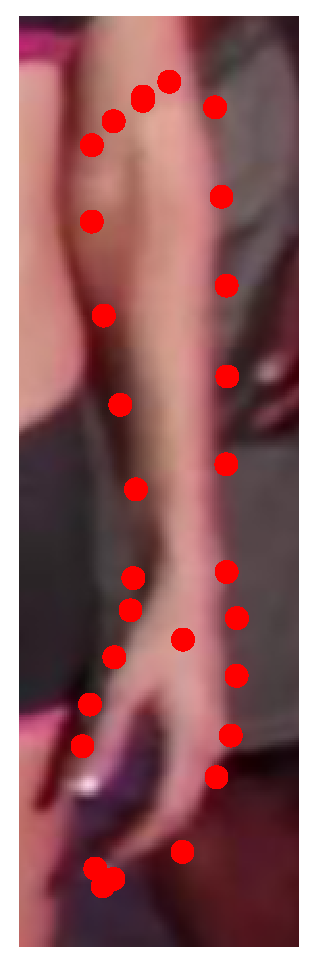
\includegraphics[height=\ofh]{resources/Fittings/35.eps}
    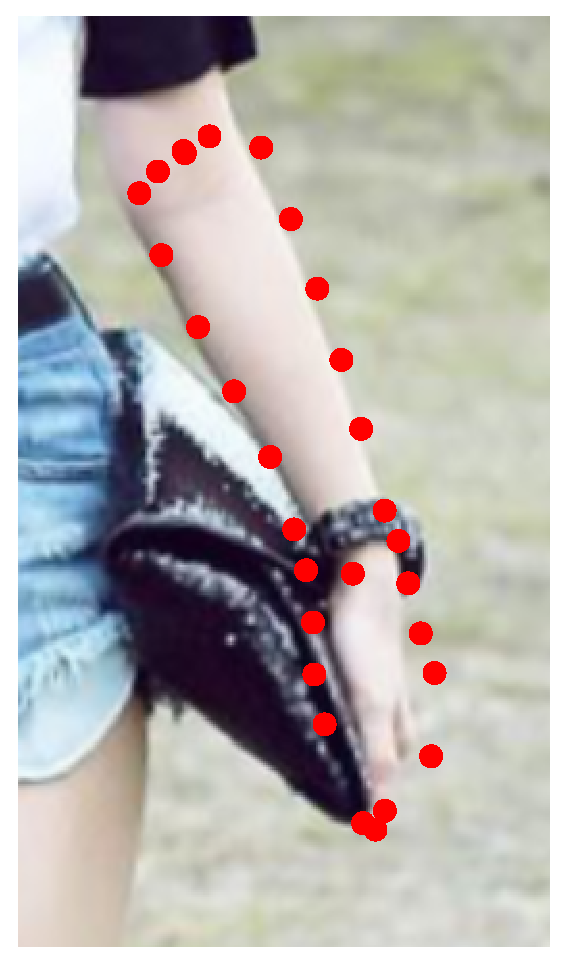
\includegraphics[height=\ofh]{resources/Fittings/36.eps}
    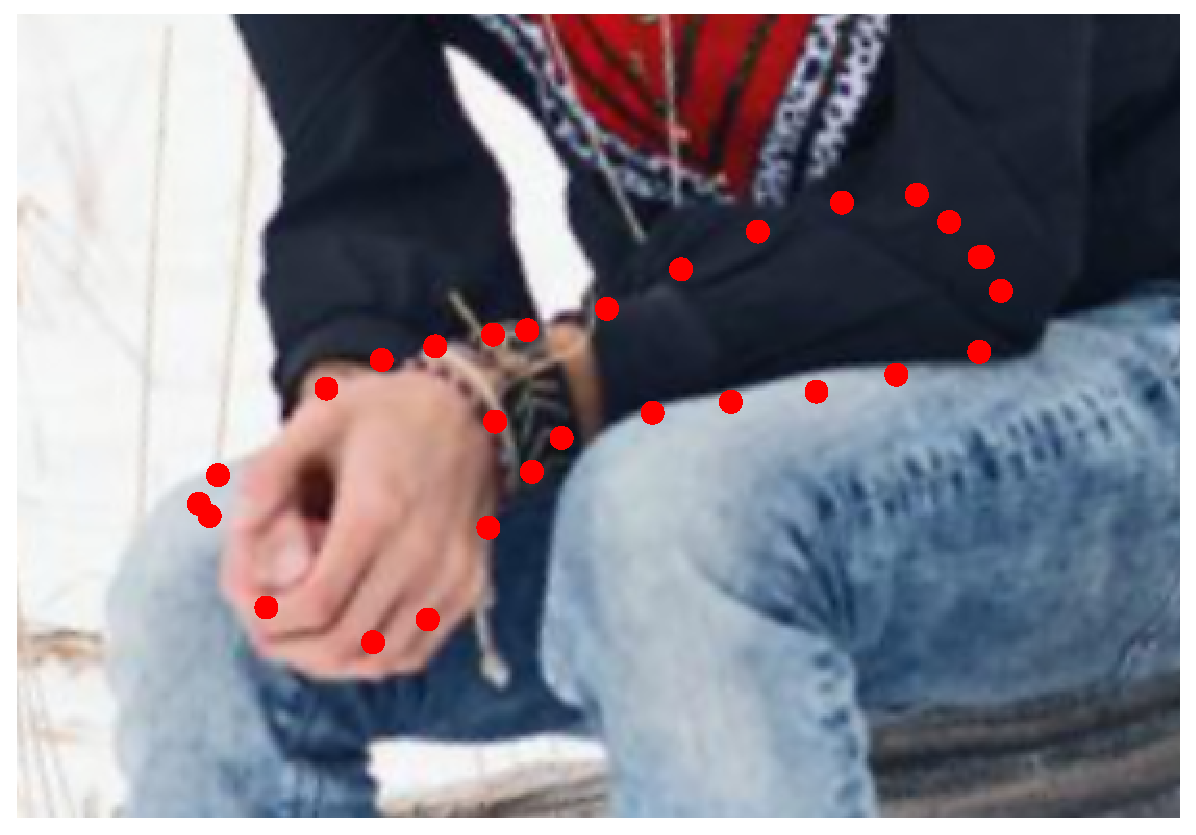
\includegraphics[height=\ofh]{resources/Fittings/37.eps}
    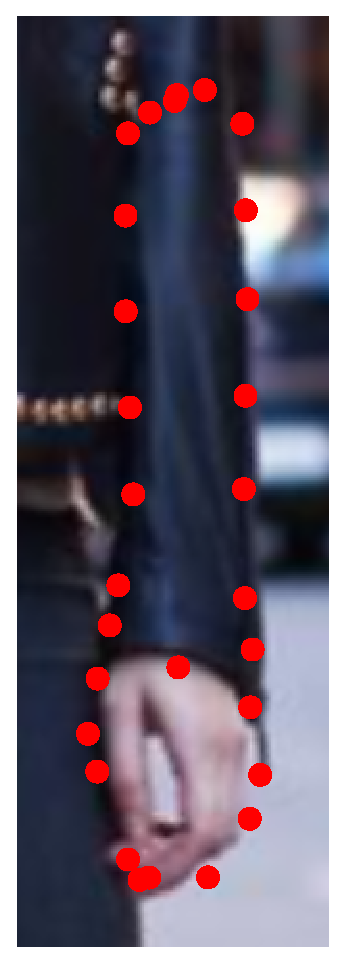
\includegraphics[height=\ofh]{resources/Fittings/38.eps}
    \includegraphics[height=\ofh]{resources/Fittings/39.eps}
    \caption{Demonstration of outline fitting of patch-based AAM on arms.}
    \label{fig:outline_fitting}
\end{figure*}

\subsection{Annotation Correction}
\label{exp:qualitative}

This experiment demonstrates inconsistency of joints annotation among MPII \cite{andriluka14cvpr}, Fashion Pose \cite{dantone2013human} and FLIC \cite{sapp2013modec}, as well as investigate the inevitable variance of manual annotation. Three well trained annotators are used to annotate left arm using 120 test images from Fashion Pose \cite{dantone2013human} dataset. Figure \ref{fig:variance} presents statistical results calculated using data annotated and officially provided with normalisation based on length of arms. Exemplar annotation visualisation also shows significant inconsistency of manual annotation on joints.

Figure \ref{exp:qualitative} presents corrections of joint annotations using patch-based SDM trained as experiment \ref{exp:benchmark}. \emph{Red} dots shows ``ground truth" points while \emph{green} dots shows landmarks after correction using our methodology. There is no doubt that points after correction show more consistency among images. Images are cropped to hand only for better visualisation.
